 \documentclass[a4paper,10pt]{article}
\usepackage[a4paper, total={6in, 8in}]{geometry}
 \usepackage{tikz}
 \usepackage{fullpage}
 \usetikzlibrary{positioning,shadows,arrows,trees,shapes,fit}
 \begin{document}
 \begin{figure}
 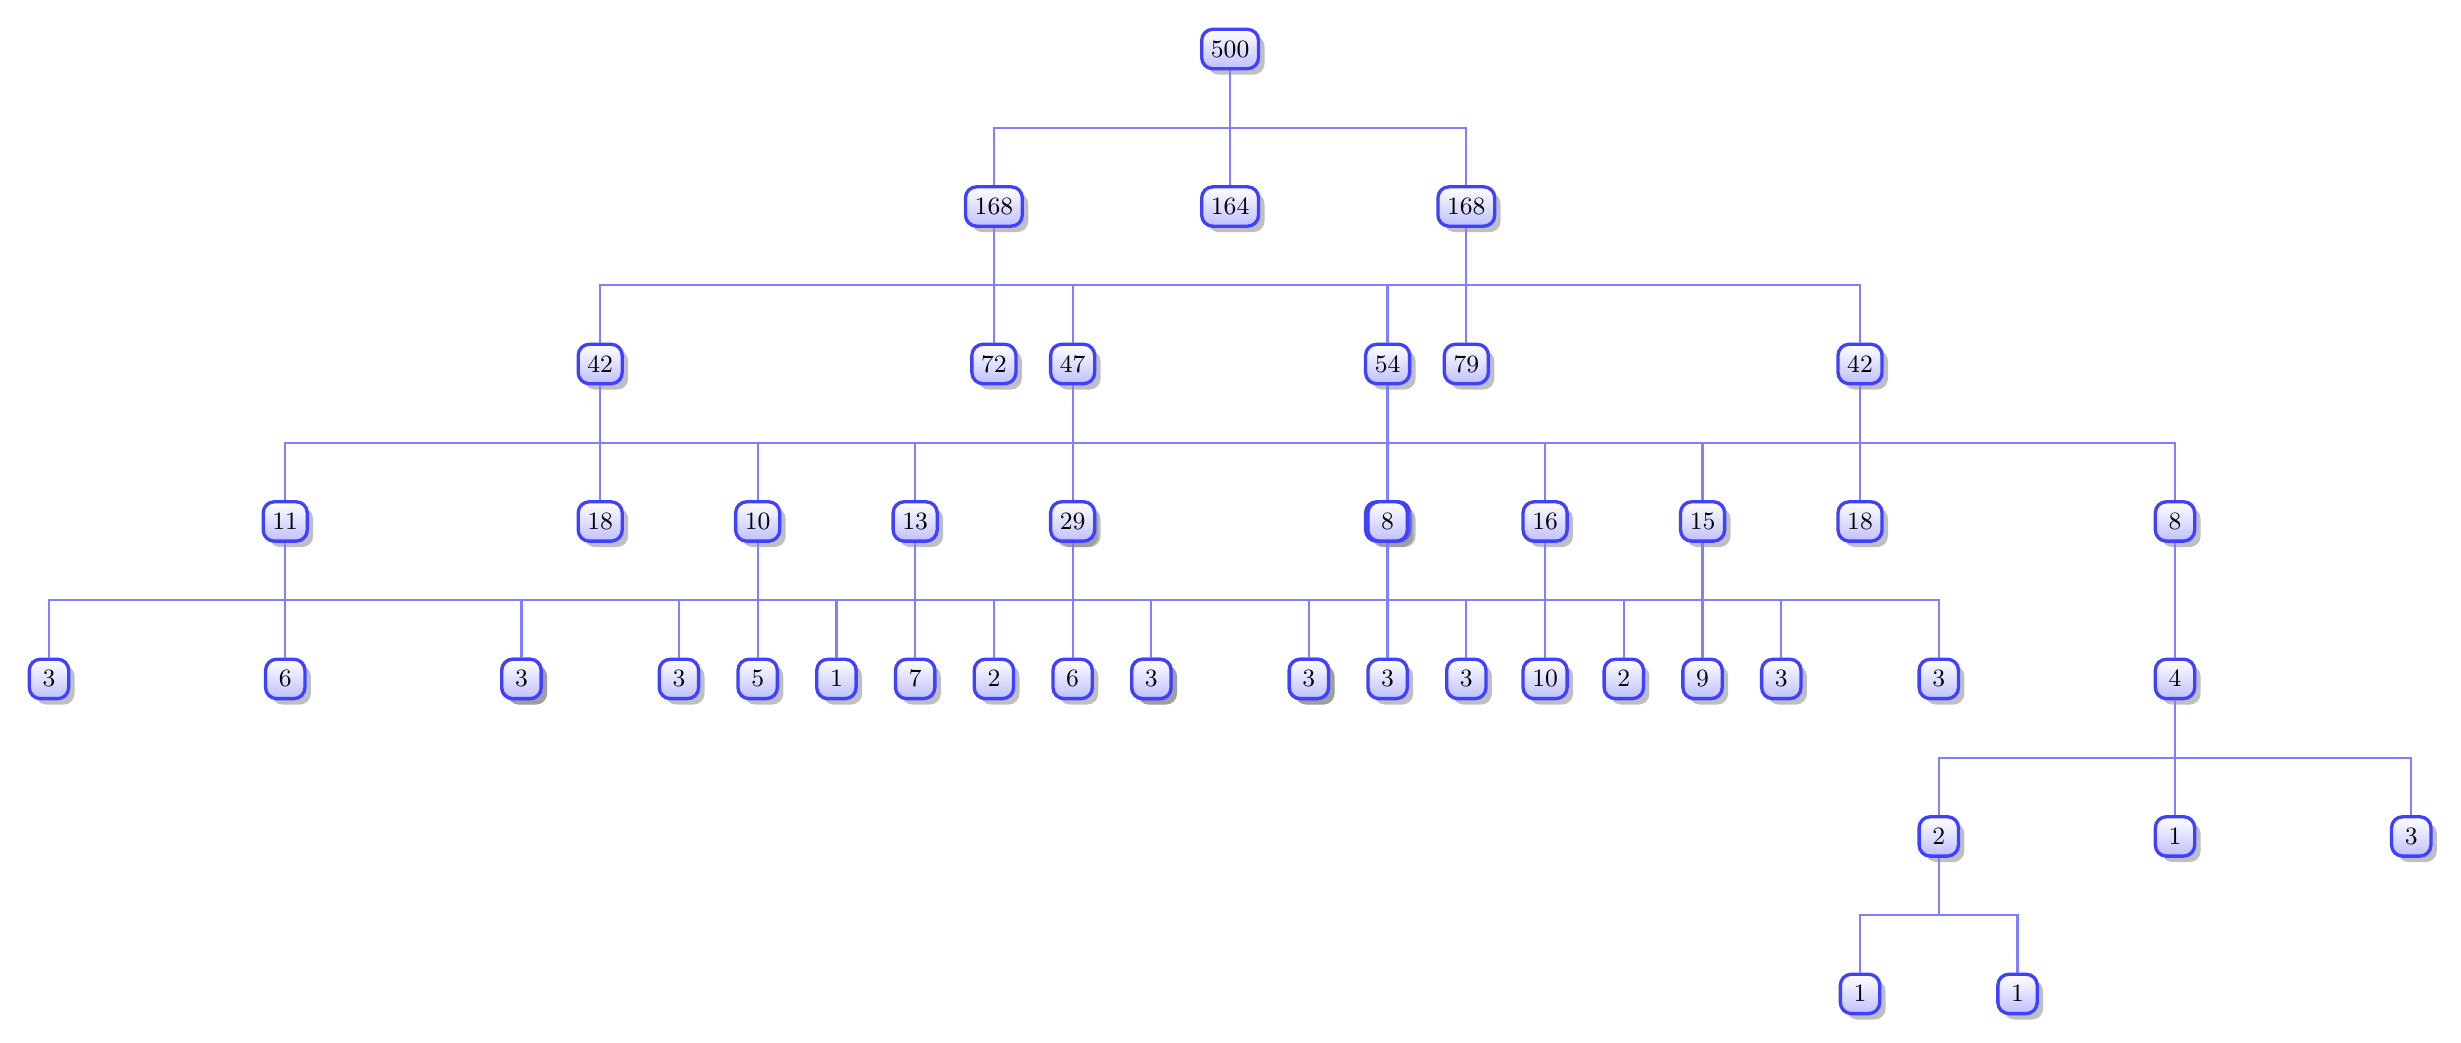
\begin{tikzpicture}
 [font=\small, edge from parent fork down, 
 every node/.style={top color=white, bottom color=blue!25, 
 	rectangle,rounded corners, minimum size=5mm, draw=blue!75,
	very thick, drop shadow, align=center},
 edge from parent/.style={draw=blue!50,thick},
 level 1/.style={sibling distance=3cm},
 level 2/.style={sibling distance=5cm}, 
 level 3/.style={sibling distance=4cm}, 
 level 4/.style={sibling distance=3cm}, 
 level 5/.style={sibling distance=3cm}, 
 level 6/.style={sibling distance=2cm}, 
 level 7/.style={sibling distance=2cm}, 
 level 8/.style={sibling distance=2cm}, 
 level distance=2cm,
 ]
\node {500} %root
child { node {168}  
child { node {42}  
child { node {11}  
child { node {3}  
 }
child { node {6}  
 }
child { node {2}  
 }
 }
child { node {18}  
 }
child { node {13}  
child { node {3}  
 }
child { node {7}  
 }
child { node {3}  
 }
 }
 }
child { node {72}  
 }
child { node {54}  
child { node {8}  
child { node {1}  
 }
child { node {6}  
 }
child { node {1}  
 }
 }
child { node {31}  
 }
child { node {15}  
child { node {3}  
 }
child { node {9}  
 }
child { node {3}  
 }
 }
 }
 }
child { node {164}  
 }
child { node {168}  
child { node {47}  
child { node {10}  
child { node {3}  
 }
child { node {5}  
 }
child { node {2}  
 }
 }
child { node {29}  
 }
child { node {8}  
child { node {3}  
 }
child { node {3}  
 }
child { node {2}  
 }
 }
 }
child { node {79}  
 }
child { node {42}  
child { node {16}  
child { node {3}  
 }
child { node {10}  
 }
child { node {3}  
 }
 }
child { node {18}  
 }
child { node {8}  
child { node {4}  
child { node {2}  
child { node {1}  }
child { node {1}  }
 }
child { node {1}  
 }
child { node {3}  
 }
 }
 }
 }
}
;\end{tikzpicture} 
 \caption{Datasize plot }  \end{figure}
\end{document} 
